\chapter{Introduction}
\label{chap:introduction}

\minitoc

\graphicspath{{.}{chapitres/introduction/}}

% software is everywhere
Nowadays software are omnipresent in people's life: banking, e-commerce, communication, etc. 
And the more and more, critical aspects such as aeronautics, voting system or even health care relies on software.

% errors can be dramatic
In one of his famous lectures~\cite{DijkstraLecture1989}, Dijkstra has stated, that in software, the following: 
\begin{center}
	\emph{``the smallest possible perturbations - \ie changes of a single bit - can have the most drastic consequences.''.}
\end{center}

Dijkstra highlights the fact that a small fault in software might affect lives.
For example, a flight crash happened in 1993 due to an error in the flight-control software of the the Swedish JAS 39 Gripen fighter aircraft.

% preventing bugs = testing tons of changes by day - CI
To avoid such situations, software editors adopted testing philosophies: the testers writes code that verify that the program is doing what the developer expects.
Over the last decade, strong unit testing has become an essential component of any serious software project, whether in industry or academia.
The agile development movement has contributed to this cultural change with the global dissemination of test-driven development techniques \cite{beck2003test}.
More recently, the DevOps movement has further strengthened the testing practice with an emphasis on continuous and automated testing \cite{Roche2013Devops}.

However, testing is tedious and costly for industries: there is no direct return to invest.
Thus, developers under pressure or by lack of discipline or time might skip the tests.

To overcome this problem, research investigates the automation of creating strong tests.
Automatic generation of tests has been well studied in the last past years~\cite{ESECFSE11, PachecoE2005}.
The dream was that a command-line would give you a complete test suite, that verifies the whole program.
For free, or almost, all the program would be well-tested.
However, studies show that developers are not using automatic test generation~\cite{TOSEM_userstudy}.
The authors investigate the truthfulness of the following hypothesis:

\emph{generating high coverage test data, we aid testers in constructing test suites capable of detecting faults.}

However, their studies showed that achieving high coverage does not necessarily improve the ability to test software.
The difficulties to understand, integrate and maintain automated test suite prevent the adoption by developers.
Also, most of the tools relies on weak or partial oracles, \eg absence of runtime errors, making them useless against bugs that do not set the program into a wrong state.

In this thesis, I aim at addressing this issue.
More precisely, the ultimate goal of this thesis is to provide an usable tool that assist developers to maintain their suite, in the context of DevOps and Continuous Integration.
To do so, I use test suite amplification, which is an emerging field, to create specific test methods according to an engineering goal.

The remaining of this section is as follow:

In \autoref{sec:intro:stamp} present the context of the thesis, the H2020 European project \emph{STAMP};

Then, I expose the roadmap of this thesis and its global vision in \autoref{sec:intro:roadmap};

Eventually, I list my publications in \autoref{sec:intro:publications} and the resulting software of this thesis in \autoref{sec:intro:software}.

\section{STAMP-project}
\label{sec:intro:stamp}

My thesis take place within STAMP, which is has been funded from the European Union's H2020 research and innovation programme under the grant agreement 731529.

STAMP stands for \textbf{S}oftware \textbf{T}esting \textbf{AMP}lification.
STAMP leverages advanced research in test generation and innovative methods of test amplification to push automation in DevOps one step further.

\begin{wrapfigure}{c}{.5\linewidth}
	\centering
	\fbox{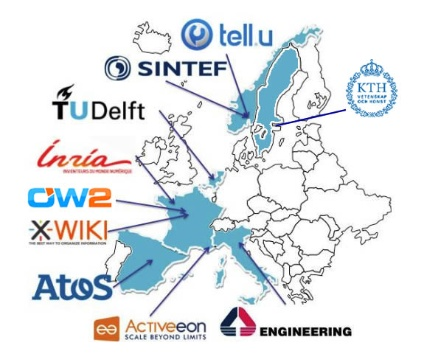
\includegraphics[width=.8\linewidth]{StampConsortiumEUMap.jpg}}
	\caption{STAMP H2020 Project Partners}
	\label{fig:intro:partners-map}
\end{wrapfigure}

Test amplification reuses existing test assets and generate more test cases and test configurations at each modification of the application.
The main goal of STAMP techniques are to reduce the number and cost of regression bugs at unit level, configuration level and production stage, by acting at all level of the development cycle.

STAMP will raise confidence and foster adoption of DevOps by the European IT industry.
The project gathers four academic partners with strong software testing expertise, five software companies (in: e-Health, Content Management, Smart Cities and Public Administration), and an open source consortium. 

This industry-near research addresses concrete, business-oriented objectives.

\subsection{Research Directions}
\label{subsec:intro:research-directions}

In STAMP, there are 3 research directions: unit testing amplification, configuration testing amplification and online testing amplification.
These 3 directions are made to be integrated in different step of the Software life-cycle, see \autoref{fig:intro:lifecyle}.

\begin{figure}[h]
	\centering
	\fbox{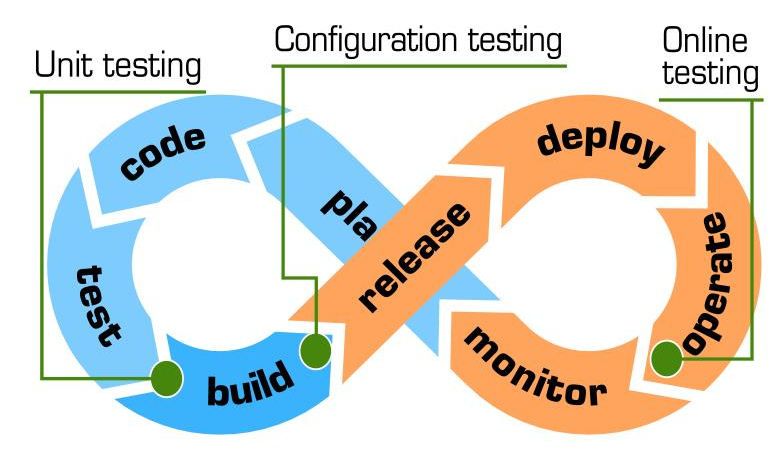
\includegraphics[width=.7\linewidth]{Workshop-intro.jpg}}
	\caption{STAMP's directions integrated in the Software life-cycle.}
	\label{fig:intro:lifecyle}
\end{figure}

\subsubsection{Unit Testing Amplification}
\label{subsubsec:intro:research-directions:unit-test-ampl}

Unit testing refers to testing small and limited part of the Software.
That is to say, it tests a single component, which has, ideally, no interference with others components.
Unit testing is a crucial part of testing since it verifies that every single component of Software does what it is expected to do.

It has two majors benefit:

1) It is easier to test and verify the behavior of a single component;

2) It allows to split the development into small part and view the system as a composition of a lot of small parts.

Unit test amplification aims at generating unit tests that are variants of existing unit tests.
These variants would improve the overall quality of unit tests according to a given engineering goal.

During my thesis, I was mainly involved in this research direction.

\subsubsection{Configuration Testing Amplification}
\label{subsubsec:intro:research-directions:config-ampl}

Configuration testing is the activity of assembling different services in a complete system, to deploy and test it, based on a pre-defined model.
Configuration testing amplification performs automatic amplification of configurations on the model, in the forms of mutation and crossover.
The goal is to create un-tested configuration to stress the Software in newly created environments.

\subsubsection{Online Amplification}
\label{subsubsec:intro:research-directions:online-ampl}

Online test amplification automatically extracts information from logs collected in production in order to generate new tests that can replicate failures, crashes, anomalies and outlier events.
This research directions aims at helping developers to debug the Software in case of crash during the production.
Debugging is a tedious task, and having a unit test method, automatically generated, would save a lot of time.

\subsection{STAMP's Output}

STAMP's final output would be micro-services that allow the developers to use STAMP's tools on their own project.
STAMP envision a web interface, on which the developers would be able to install, configure and execute the tools.
Also, the developers would be able to manage the output of these executions and link them directly to their project, \eg integrate an amplified unit test into their test suite.

\section{Dissertation Roadmap}
\label{sec:intro:roadmap}

\begin{figure}[h]
	\centering
	\fbox{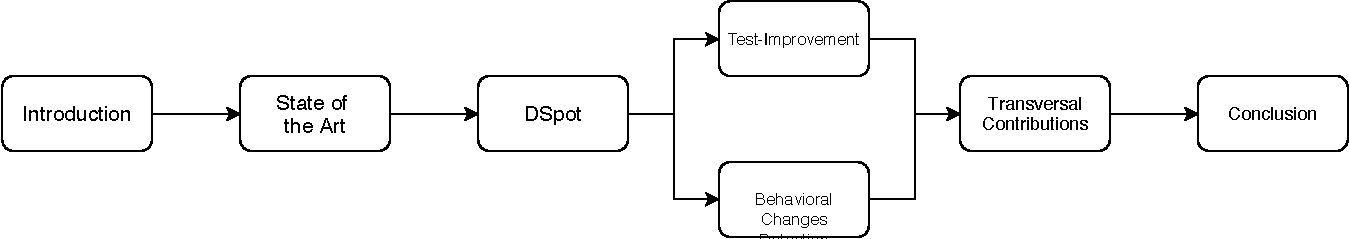
\includegraphics[width=\linewidth]{roadmap.pdf}}
	\caption{Dissertation Roadmap}
	\label{fig:intro:roadmap}
\end{figure}

This thesis is divided into 6 chapters.

First, \autoref{chap:sota} exposes the state of the art of test amplification.

Then, \autoref{chap:dspot} gives the detail of the major technical contributions of this thesis: \dspot.

\autoref{chap:test-improvement} and \autoref{chap:dci} relate two evaluations of \dspot on open-source projects from \gh.
Each of these evaluations has their own characteristics, novelties and motivations.

During my thesis, I developed a lot of skills that allowed me to participate to transversal contributions. 
These contributions are related in \autoref{chap:transversal-contributions}.

Eventually in \autoref{chap:conclusion}, I conclude and give the short- and long-term perspectives.

\autoref{fig:intro:roadmap} summarizes the roadmap.

\section{Publications}
\label{sec:intro:publications}

\section{Software and Impact On The Community}
\label{sec:intro:software}

